\begin{figure}[!htpb]
	\hypertarget{fig:actualizacionXmlLineaBase}{\hspace{1pt}}
	\begin{center}
		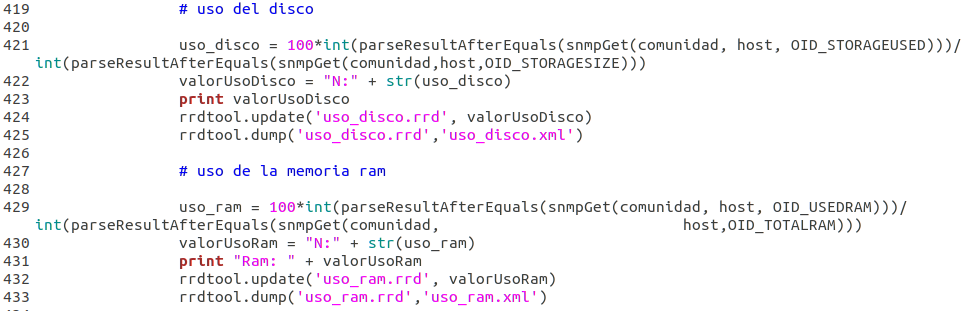
\includegraphics[width=0.7\textwidth]{imagenes/LineaBase/actualizacionXmlLineaBase.png}
		\caption{Fragmento de código que actualiza los datos en el XML.}
		\label{fig:actualizacionXmlLineaBase}	
	\end{center}
\end{figure}


\begin{figure}[!htpb]
	\hypertarget{fig:creacionImagenLineaBase}{\hspace{1pt}}
	\begin{center}
		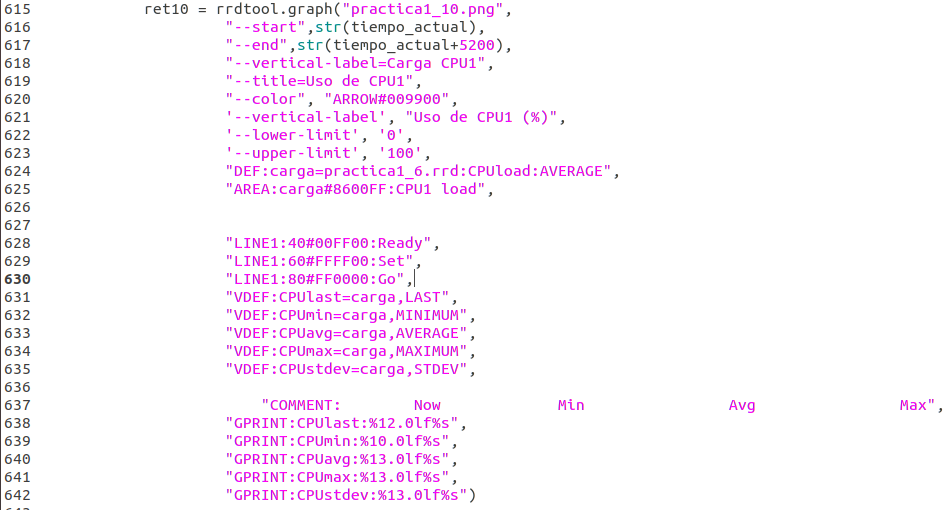
\includegraphics[width=0.7\textwidth]{imagenes/LineaBase/creacionImagenLineaBase.png}
		\caption{Fragmento de código que crea la imagen que mostrará la gráfica.}
		\label{fig:creacionImagenLineaBase}	
	\end{center}
\end{figure}


\begin{figure}[!htpb]
	\hypertarget{fig:envioAlertaLineaBase}{\hspace{1pt}}
	\begin{center}
		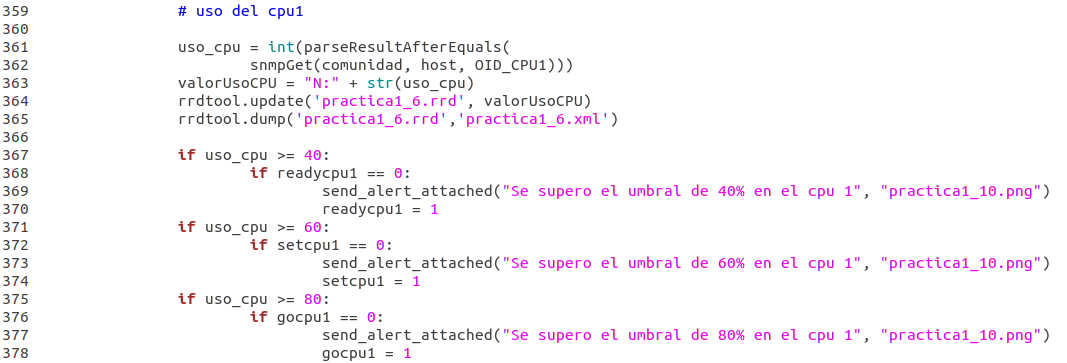
\includegraphics[width=0.7\textwidth]{imagenes/LineaBase/envioAlertaLineaBase.png}
		\caption{Fragmento de código que sirve para saber cuándo alertar que está pasándose de la línea de base.}
		\label{fig:envioAlertaLineaBase}	
	\end{center}
\end{figure}


\begin{figure}[!htpb]
	\hypertarget{fig:practica1_10}{\hspace{1pt}}
	\begin{center}
		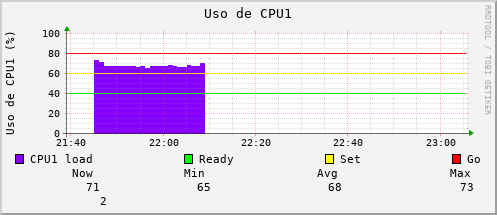
\includegraphics{imagenes/LineaBase/practica1_10.png}
		\caption{Uso del CPU 1 mostrando también las líneas que indican los límites.}
		\label{fig:practica1_10}	
	\end{center}
\end{figure}


\begin{figure}[!htpb]
	\hypertarget{fig:practica1_11}{\hspace{1pt}}
	\begin{center}
		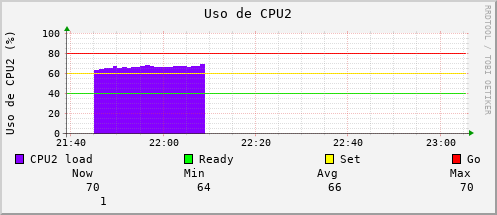
\includegraphics{imagenes/LineaBase/practica1_11.png}
		\caption{Uso del CPU 2 mostrando también las líneas que indican los límites.}
		\label{fig:practica1_11}	
	\end{center}
\end{figure}


\begin{figure}[!htpb]
	\hypertarget{fig:uso_disco}{\hspace{1pt}}
	\begin{center}
		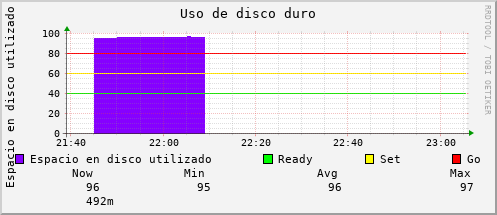
\includegraphics{imagenes/LineaBase/uso_disco.png}
		\caption{Se muestra el uso del disco así como las líneas que indican los límites.}
		\label{fig:uso_disco}	
	\end{center}
\end{figure}

\pagebreak
\begin{figure}[!htpb]
	\hypertarget{fig:uso_ram}{\hspace{1pt}}
	\begin{center}
		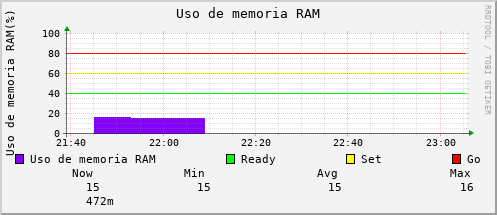
\includegraphics{imagenes/LineaBase/uso_ram.png}
		\caption{Se muestra el uso de la RAM así como las líneas que indican los límites.}
		\label{fig:uso_ram}	
	\end{center}
\end{figure}